\documentclass[20pt,xcolor={dvipsnames}]{beamer}

\usepackage{amsmath}%
\usepackage{amsfonts}%
\usepackage{amssymb}%
\usepackage{caption}
\usepackage{subcaption}
\usepackage{tikz}
\usepackage{txfonts}
\usepackage{multirow}
\usepackage[percent]{overpic}
\usepackage{textcomp}

% wielkosc liter
\usepackage{relsize}

%------------------------------------------------------------------
\hfuzz20pt % Don't bother to report overfull boxes < 5pt

\pagestyle{plain} % plain/empty
\definecolor{MyFavourite}{RGB}{34, 139, 34}
\definecolor{MyRed}{RGB}{205,38,38}
\setbeamercolor{normal text}{fg=MyFavourite,bg=black}
\setbeamercolor*{enumerate item}{fg=MyFavourite}
%\setbeamersize{\hoffset = 0pt}
%\addtobeamertemplate{frametitle}{\vspace{5cm}}
\pagecolor{black}
\usetikzlibrary{positioning}

\newcommand{\heart}{\ensuremath\varheartsuit}
\newcommand{\myitem}[1]{\setbeamercolor{item}{fg=MyFavourite}\item #1} 

% remove page numbering
\makeatletter
\let\@oddfoot\@empty
\let\@evenfoot\@empty
\makeatother

%%% --------------------------------------------------------------
\begin{document}

\begin{frame}[c]

\centering

\scalebox{0.3}{\includegraphics{logo5}}

\vspace{-1cm}

\Huge Infermath

\normalsize Open source of math 

\end{frame}


\begin{frame}[c]

\LARGE

Quantitative \\
Easing \\
\vspace{0.5cm}
\normalsize
\onslide<2->{trillion = million of millions \textdollar \texteuro  \textyen}

\end{frame}

\begin{frame}[c]

\centering

\LARGE

\centering
Bond \\

\vspace{0.5cm}
\onslide<2->{\scalebox{0.07}{\includegraphics{chain}}} \\
\vspace{0.5cm}

\begin{overlayarea}{\textwidth}{\textheight}
	\centering
	\only<3>{Word}
	\only<4>{Obligation}
\end{overlayarea}

\end{frame}

\begin{frame}

\centering
\Large
Bond Issuers
\normalsize

\vspace{1cm}

\begin{columns} 

\onslide<3->
\column{0.3\textwidth}
\centering
\includegraphics[height=3cm]{factory} \\
Corporates

\onslide<2->
\column{0.4\textwidth}
\centering
\includegraphics[height=3cm]{capitol} \\
Governments

\onslide<4->
\column{0.3\textwidth}
\centering
\includegraphics[height=3cm]{bank} \\
Banks

\end{columns}

\end{frame}


\begin{frame}%[c]

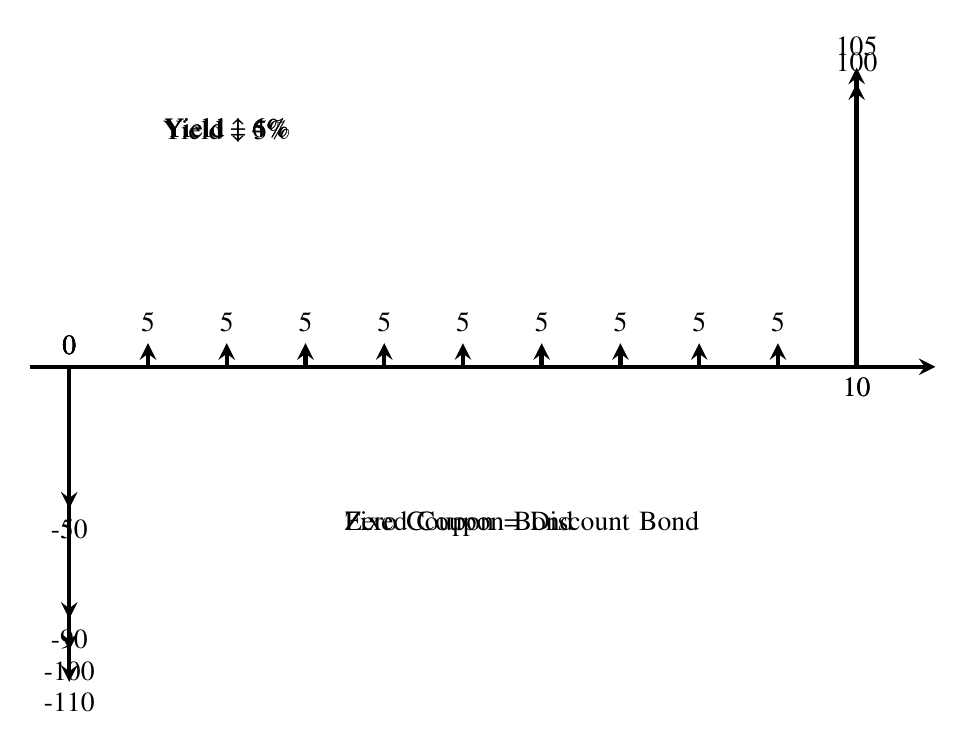
\begin{tikzpicture}[>=stealth,ultra thick]

    \draw[->] (-0.5,0) -- (11,0);
		
		\onslide<2-3,6-8>
		\draw [->] (0,0) node[above] {0} -- (0,-3.6) node[below] {-100};
		
		\onslide<3-6>
		\draw [->](10,0) node[below] {10} -- (10,3.6) node[above] {100};
		
		\onslide<4-5>
		\draw [->] (0,0) node[above] {0} -- (0,-1.8) node[below] {-50};
		
		\onslide<5>
		\draw(6,-2) node [text width =5cm]{Zero Coupon = Discount Bond};
		
		\onslide<6->
		\draw(6,-2) node [text width =5cm]{Fixed Coupon Bond};
		
		\onslide<7->
		\draw [->](10,0) node[below] {10} -- (10,3.8) node[above] {105};
    \foreach \x in {1,...,9}
		\draw [->](\x,0) -- (\x,0.3) node[above] {5};
		
		\onslide<8-9>
		\draw(2,3) node {Yield = 5\%};
		
		\onslide<10-11>
		\draw(2,3) node {Yield $\uparrow$ 6\%};
		
		\onslide<9-10>
		\draw [->] (0,0) node[above] {0} -- (0,-3.2) node[below] {-90};
		
		\onslide<12->
		\draw(2,3) node {Yield $\downarrow$ 4\%};

		\onslide<11->
		\draw [->] (0,0) node[above] {0} -- (0,-4) node[below] {-110};
		
\end{tikzpicture}

\end{frame}

\begin{frame}[c]

\centering

\scalebox{0.3}{\includegraphics{logo5}}

\vspace{-1cm}

\Huge Infermath

\normalsize Open source of math 

\end{frame}

\begin{frame}[c]

\centering
\onslide<3->{Interest rate - r}

\vspace{-1cm}

\begin{align*}
100 \onslide<2->{&=90} \onslide<3->{+90r}\\
\onslide<4->{100&=90(1+r)} \\
\onslide<5->{1+r&=100/90} \\
\onslide<6->{r&=100/90 - 1} \\
\onslide<7->{r&=11.11\%}
\end{align*}

\end{frame}

\begin{frame}[c]

\centering
Annual interest rate

\vspace{-1cm}

\begin{align*}
\onslide<5->{100&=} \onslide<2->{90} \onslide<3->{(1+r)} \onslide<4->{(1+r)}\\
\onslide<6->{100&=90(1+r)^2} \\
\onslide<7->{(1+r)^2&=100/90} \\
\onslide<8->{r&=\sqrt{100/90} - 1} \\
\onslide<9->{r&=5.41\%}
\end{align*}

\end{frame}

\begin{frame}[c]

\centering
General case

\vspace{-1cm}

\begin{align*}
\onslide<2->{100&=90(1+r)^{10}} \\
\onslide<3->{Notional &= Price(1+r)^n} \\
\onslide<4->{(1+r)^n&=Notional/Price} \\
\onslide<5->{r&=(Notional/Price)^{1/n} - 1} 
\end{align*}

\end{frame}

\begin{frame}[c]

\centering

\begin{align*}
Notional &= Price (1+r)^{n} \\
\onslide<3->{PV &= Price} \\
\onslide<4->{FV &= Notional} \\
\onslide<5->{Price &=Notional  \cdot \frac{1}{ (1+r)^{n} }} \\
\onslide<2->{PV &=FV \cdot DF } \\
\onslide<7->{DF &= \frac{1}{ (1+r)^{n} }}
\end{align*}


\end{frame}


\begin{frame}[c]

\centering

\begin{equation*}
\underset{Value}{\underset{Present}{\scalebox{3}{PV}}} \onslide<2->{\scalebox{3}{=}
\underset{Value}{\underset{Future}{\scalebox{3}{FV}}}} \onslide<3->{  \scalebox{3}{$\cdot$}
\underset{Factor}{\underset{Discount}{\scalebox{3}{DF}}}}
\end{equation*}

\end{frame}


\begin{frame}

\vspace{-1cm}
\hspace{-0.5cm}
\Huge Fixed Income

\vspace{1cm}

\begin{columns}

\column{0.7\textwidth}
Debt  \\ Concept

\column{0.3\textwidth}
\scalebox{3}{\color{MyRed} 1}

\end{columns}

\end{frame}

\begin{frame}

\vspace{-1cm}
\hspace{-0.5cm}
\Huge Fixed Income

\vspace{1cm}

\begin{columns}

\column{0.7\textwidth}
Debt  \\ Valuation

\column{0.3\textwidth}
\scalebox{3}{\color{MyRed} 1}

\end{columns}

\end{frame}

\begin{frame}

\centering
\huge

\begin{columns}
\column{0.5\textwidth}
Bonds  \\ Concept
\column{0.5\textwidth}
\includegraphics[height=5cm]{chain} 
\end{columns}

\vspace{0.25cm}

Fixed Income

\end{frame}

\begin{frame}[c]

\centering

\scalebox{0.3}{\includegraphics{logo5}}

\vspace{-1cm}

\Huge Infermath 

\normalsize Open source of math 

\vspace{1cm}

\large www.infermath.com \\
www.facebook.com/infermath 

\end{frame}

\end{document}


